\chapter{Gregorian chant}

\emph{This chapter is adapted after \cite{chant_book}.}

In order to design an application that processes chant data, it is necessary to understand the basics of what Gregorian chant is.

Gregorian chant is the music associated with the Roman catholic tradition. It is sung in churches, as well as in convents, and can also be sung during outdoor
ceremonies such as processionals (and outdoor liturgy in general.). Its current written form is, as far as we can tell, very similar to its original
form from the first millenium.

Gregorian chant is one of the earliest forms of music preserved in written form, and the
largest preserved body of medieval music. The earliest preserved fragments of written notes date back to the 9th century, although texts from as early as 
the eighth century have been found.. Its name, Gregorian, references Pope Gregory the Great, however, his relation to the chant is not entirely clear.

It is not the only type of chant. In the early centuries after Christianity spread across Western and Eastern Roman Empire,
new forms of worship started being developed. The most obvious differences were between the West and the East, which had multiple cultural
centers such as Constantinople, Jerusalem, or Alexandria. However, liturgies varied in the West as well, from Rome to Milan to the Iberian peninsula to Gaul.
Each center developed their own tradition, including their own type of chant. Roman-catholic tradition being so prevalent in Europe
can be attributed to Charlemagne's attempt to unify European kingdoms.

Gregorian chant is an integral part of the Roman church, and has been so for centuries. It is the monophonic music (i.e. single-voice)
sung during liturgy at specific points, defined by the rules for conducting liturgy according to the Roman rite (the rite of the Latin church, or what
we know as the Catholic church today). Here, liturgy means chant sung during Christian worship. Unlike in the Eastern churches, where the term is reserved 
for the Eucharist, liturgy includes both the Mass and the Divine Office in the Roman church.

As with other kinds of music, there exist several genres of Gregorian chant. A \emph{genre} is a group of chants that share some characteristics, such as
complexity or content. Different genres play different roles in the liturgy. Some are sung while the priest is walking to the altar, others convey the
core message of a mass, others have just a decorative purpose.

Not all genres are sung during every kind of worship. In the following section, we describe the Mass and the Divine Office and mention some genres
that are specific for each.

\section{Mass and Divine Office}

Mass is the service most familiar to most believers.
It can be divided into several parts, all leading up to the most important one, the act of communion. This act commemorates the Last Supper,
Jesus's last meal with his disciples before his execution. During the communion, bread, representing Christ's body, and wine, representing his
blood, are given out. During the course of the Mass, multiple different chants are sung. \emph{Introitus}, meaning 'entrance', is sung at the beginning
of the service while the priest and his assistants are walking to the altar. \emph{Tractus} is a chant that is sung during Lent, i.e. the period
between Ash Wednesday and the Saturday before Easter. Outside of this period, \emph{alleluia} replaces \emph{tractus} and is followed by \emph{sequentia}
on the most important feast days.

The other part of the liturgy, besides the Mass, is the Divine Office, also called Liturgy of the Hours or canonical hours. It is the set of chants
sung during services at different times of the day, for example \emph{Vespers} in the evening or \emph{Lauds} in the morning. The office consists
largely of singing psalms, of which there are 150, all sung on different days and hours. Psalms were usually preceded and followed by antiphons,
which differ not only by the day of the week, but also depending on the position within the liturgical year. Each day of the week had an allocated
set of antiphons, hymns and responsories, while responsories were assigned to the different Sundays. Additionally, important feasts had their own
set of chants to be sung.

The liturgical year consists of many feasts. Some feasts are fixed on a specific date. Feasts associated with a specific saint are an example of those.
For example, John the Baptist is celebrated on the 24th of June, Michael on the 29th of September, and All Saints on the 1st of November. Other
fixed-date feasts include Christmas Day (25 December), Epiphany (6 January), and others. Such feasts can fall on any day of the week, and if they fall
on a Sunday, they will take precedence over it. On the other hand, there are also feasts that are fixed to a specific day of the week, the most important
of them being Easter Sunday, the day when Christ rose from the dead. Each feast has a different set of chants that can be completely original.

\section{Variation between chants}

The individual chants differ in several criteria, the first one being the \emph{mode}. Mode is the system of pitch organization, somewhat similar to modern-day
scales. All chants use the seven tones of a diatonic scale, meaning a scale with five whole steps and two half steps.

Melodies are classified into one of eight modes according to their last note, called \emph{finalis}, and their range. Most chants
end on one of the notes \emph{D}, \emph{E}, \emph{F}, or \emph{G}. These four notes determine four pairs of modes. The melodies were further classified
depending on whether they moved mostly in the range above the \emph{finalis}, in which case it would be classified as the \emph{authentic} mode
of the pair, or in the range around the \emph{finalis}, which means it is classified as the \emph{plagal} mode. Some types of chant tend to
occur mostly in a specific mode.

\begin{figure}[h]
\centering
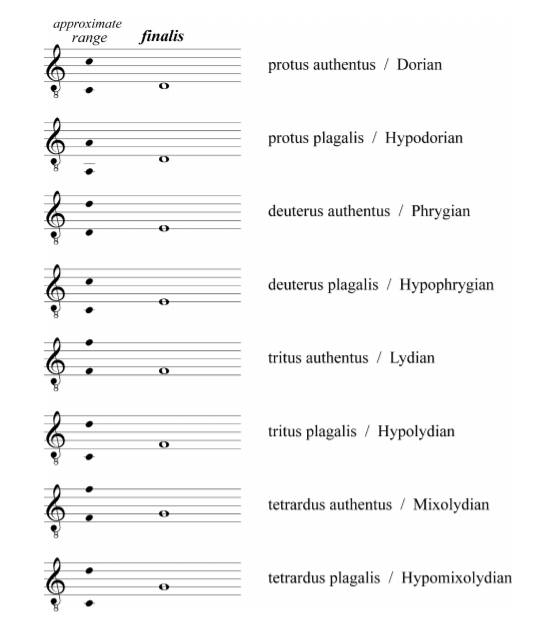
\includegraphics[scale=0.7]{modes}
\caption{List of modes, their ranges and finalis. \cite[p.~44]{chant_book}}
\end{figure}

Another criterion is the complexity of chants, that is, how elaborate the melody is. On the one side of the spectrum, there is a one-to-one
syllable to note correspondence. Antiphons and some hymns are genres close to this text-setting. The other extreme is melismatic style. Melisma
is a long vocalization of a single syllable, therefore melismatic melodies are more ornate. Some of the more melismatic genres are the gradual,
tract and offertory.

We have already mentioned several different genres of chant. Antiphons are chants sung to frame a psalm during the Office hours. They are relatively
short and simple, somtimes consisting of only two phrases. Responsories are sung during the Night Office. Each has a main section and a verse. They are
melodically very rich and are on of the most impressive forms of chant. The number of chants sung during the Mass is lower, as there will usually
only be one introit, one gradual, etc. during a service.

It is important to note that text and melody do not form unique pairs. Instead, each text
can be sung to multiple different melodies and multiple texts can be sung to one melody. Chants with the same melody but different lyrics
are called \emph{contrafacta}.

\section{Chant notation}
\label{section:notation}

It is clear that the annual cycle is very complex and the amount of chants is abundant. Therefore, it is not surprising that while the chants during the
services themselves were sung from memory, they were written down in books. Each church and each convent had their own manuscripts, which is the
reason of their abundance.

At first, melodies were written without a staff. The writers simply marked the direction in which the pitch was moving, serving barely as memory aids,
not for learning. Later, better accuracy was required,
therefore melodies started being written with their exact pitch, resembling the modern-day musical notation. However, written melodies never contained
explicit information about the rhythm. An example of a chant melody as found in a manuscript is shown in Figure \ref{fig:chant}.

\begin{figure}[h]
\centering
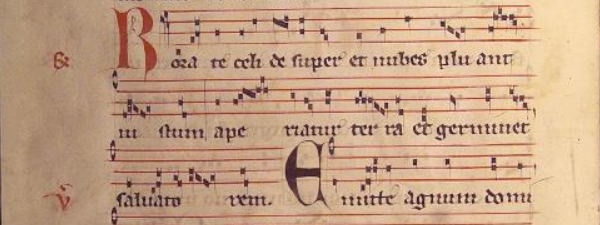
\includegraphics{manuscript}
\caption{Example of a chant in a manuscript. \cite[id~007553]{cantus_db}}
\label{fig:chant}
\end{figure}

In the middle ages, tools to tune singers' voice to a specific pitch were not readily available. This led to the singing ``by feeling''. As a result,
some churches or convents sang the same melody, but shifted by a certain interval, and they were inscribed in manuscripts with this shift. Such melodies
(those that differ by the same interval in all positions) are called \emph{transpositions}.

\section{Digital chant research}

The study of Gregorian chant is an active area of musicology covering many centuries and the whole continent. It has a rich digital infrastructure facilitating
the research using computational methods. There exist several large databases of digitalized chants, such as the Cantus database\footnote{\url{https://cantus.uwaterloo.ca/}},
and the databases are indexed in the Cantus Index,\footnote{\url{http://cantusindex.org/}}, providing a standard API for searching among them.

There are several problems that can be tackled using computational methods. For example, some researchers have a sense that women's houses may have used
transposed modes more frequently than men's houses. However, no research has been done on this topic yet, as it requires comparing too many chants to draw
a conclusion with reasonable scientific certainty. Computational methods could help quantify the numbers.
Another question is whether mode distribution is different according to monastic order. It is also possible to find if there is a regional preference for
pitch progression (e.g. A-B-A vs. A-C-A) by comparing manuscripts.\footnote{From personal communication with Debra Lacoste and Jennifer Bain.}

These are examples of problems that have not been properly researched yet, but the digitalization of resources makes the research feasible.
